\thispagestyle{empty}
 \begin{center}
{\bf \TITLE}\\
{
%Tim Menzies, IEEE Fellow, NC State
}
 \end{center}
\vspace{-3mm}
\noindent
%(In this section, all terms shown in {\bf {\em bold font}} are explained later in this proposal.)

\section{Introduction}  Zhu, Whittle, et al.~\cite{Zhu2022} say that transparency, and the ability to audit complex AI models, are an essential component of 
responsible AI. 
Ben Green~\cite{green2022flaws} notes that many recent policies      require humans review   to assess the decisions from software models.  
When the expertise required for   reviewing is in short supply,     reviews cannot be a human-in-the-loop review of each decision. Rather,   reviews must take the form of some committee
representing {\em stakeholder\footnote{``Stakeholders'' 
are individual or organization having a right, share, claim, or interest in a system or in its possession of characteristics that meet their needs and expectations (ISO/IEC/IEEE 2015~\cite{iso2015systems}).}}
making
{\em occasional audits} (e.g. every week, month, or year). We assume   {\em occasional audits}
since  the  personnel    serving on these audit committees are experts in their field-- which means
that their services are required for  many things  (not just auditing). Hence, 
 audits only occur {\em occasionally}  when those experts can find time
away from their other commitments. 

The problem with   {\em occasional audits} is that while these might occur {\em weekly, monthly, etc}, 
new   hyperparameter optimizers (discussed below) can   update models in {\em minutes, hours, days}.
That means that models change faster than they can be occasionally audited.
(discussed below) which mean it is now becoming   fast to tune deep learning  models.
Does this mean we need to  force humans to continually audit models? Perhaps not.
We propose {\IT} which combines two types of tools to support  occasional  audits {\em as well as} offering some   guarantee
across the space of changes between the audits:  
\bi
\item {\em Audit Tools Type1 (intra-audit):}
  test if a  model is  fair on {\em past cases} by     tunomg the learners  to optimize for multiple stakeholder goals
as well as goals that measure bias and discrimination;
 compare the tuned learner to the original learner;  then recommend a review of   past cases that performed poorly on the original learner, but significantly better on the tuned learner. 
\item {\em Audit Tools Type2 (inter-audit):}
given the tunings from part1, generate {\em worst-case counterfactuals}; i.e. the least change to current data that most reduces performance (as measured by stakeholder goals).   The audit team could    then conclude  that until the model
is extended to cover these worst cases, it must be  policy   never to process  anything like those counterfactuals. 
\ei
{\IT} is novel not just for the {\em Type2} work, but also for the multi-objective nature of {\em Type1}.
Much current work in AI model
robustness focuses just on {\em Type 1}, and only for a single goal such as accuracy (e.g ~\cite{diffenderfer2021winning}).
But in {\IT}, we assume stakeholder care about  a wide variety of domain-specific goals.
We claim that:
\begin{formal}\noindent
 \underline{\bf Stakeholders}  team (i.e. non-technical representatives from  many
 social groups) can \underline{\bf quickly audit}, fault and/or certify   
 \underline{\bf deep learning
models}   via tools which, under-the-hood, using (a)~knowledge distillation, (b)~semi-supervised learning , (c)~landscape
analysis,   and  (d)~multi-objective optimization.\end{formal}
\noindent
 To test this claim, we will perform human studies with {\IT} and 
stakeholders to see how quickly (if at all), they can find seeded faults in ML models.
When evaluating this claim, the term \underline{\em quickly} will become important since 
the experts serving on these audit teams are typically working under strict time constraints
(since they need to get back to their other duties).  

Our pre-experimental belief is that all the   technologies mentioned in our claim are necessary for {\IT}.
Once deep learner {\em distillers} condense the overall search space, we can dividing the model review problem into several simpler task of  reviewing of several small models.
Also,
our (b)~{\em semi-supervised learners}, combined with (c)~{\em landscape analysis}, will allow stakeholders to  ignore   less-informative regions of the models.
Further,
our (d)~{\em multi-objective optimizers} will 
let stakeholders trade off between competing goals. To assess this pre-experimental belief,
we will   conduct ablation
studies~\cite{cohen1995empirical} where each of these (a)(b)(c)(d) will be removed from {\IT}, and the performance of the ablated system will be compared to the whole. 

\section{Background and Motivation}
Green~\cite{green2022flaws}  warns us that {\em
        ..people (including experts) are susceptible to 'automation bias' (involving)  omission errors—failing to take action because the automated system did not provide an alert—and commission error''}. 
        Sadly,
there are   many recent examples   where  ML-models would have benefited from more effective auditing. 
   For example,  it took years to realize that (in)famous
COMPAS  model had an alarming difference in the false alarm rates for black and white defendants~\cite{Chakraborty2020artifact}. 
Facial recognition software   predicting    gender \& age have a much
higher error rate for dark-skinned women~\cite{Skin_Bias}.
  Amazon's   software for same-day delivery   is known to be   biased against black neighborhoods \cite{Amazon_Bias}. 
 Earlier versions of Google Translate  has gender bias
 (e.g. ``She is an engineer, He is a nurse''   translated to  Turkish then
  back to  English gives ``He is an engineer, She is a nurse''~\cite{Caliskan183}). 
Rudin~\cite{rudin2019explaining}, 
Nobel~\cite{noble2018algorithms} and Gebru~\cite{gebru21} list other examples.
When   audit policies routinely miss important problems,  Green remarks that  this   can lead to the reverse of their desired effect  by {\em ``legitimizing the use of   faulty and controversial algorithms without addressing (their fundamental issues''}~\cite{green2022flaws}. 

 


 
\begin{wrapfigure}{r}{2in}
\centerline{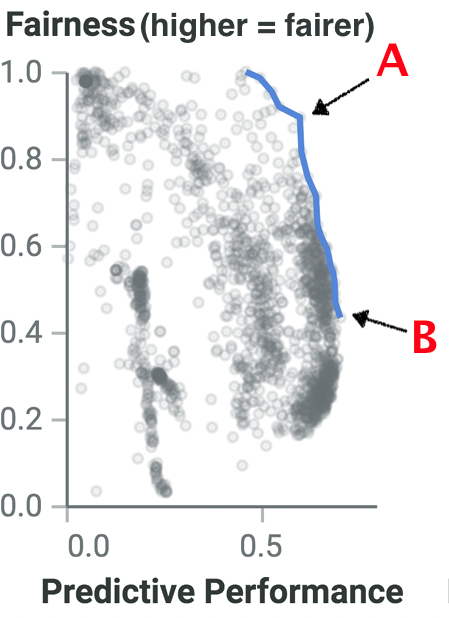
\includegraphics[width=1.5in]{fig/aof.png}}
\caption{Effect of 10,000   tunings
on predicting \underline{\em account opening fraud}.
X-axis= accuracy.
Y-axis= ratio of false positives   men:women.
Learners=
random forest;   regression;   boosted trees; simple decision trees;  a feed-forward NN.
From~\cite{F_Cruz_2021}.}\label{one}\end{wrapfigure}
In many ML models, performance bugs in models learned via machine learning can be addressed via tuning
the control parameters of that model\footnote{For neural networks, those learners can tune many parameters including the
sample shown in 
in Table~\ref{cnn1}.B}
\footnote{For nearest neighbor classification, those algorithms have many tuning options
including (a)~how   to measure
distance; (b)~how many neighbors to consider; (c)~how to combine the influences of those neighbors;
(d)~how (or if) to pre-cluster
the data (in order to optimizer the neighborhood lookup); etc.} 
\footnote{For Random Forests,   those   learners
can tune
(a)~how many $T$ decision trees to build (e.g. $T\in \{10,20,40,80,160\}$); (b)~how many features $F$
to use for each tree (e.g. $F \in{2,4,10,20,
\mathit{sqrt}, \mathit{log2}, \mathit{all}}$);
(c)~what voting measure should be used to poll the whole forest (e.g. {\em majority} or {\em weighted majority}); 
(d)~what impurity measures (e.g. {\em gini} or {\em entropy} or {\em log.loss}); (e)~what is the minimum examples needed to branch a sub-tree
(e.g. {\em min}$\in \{2,5,10,20,50,100\}$; (f)~should branches be {\em binary} or {\em n-arty}.
In all, this gives us
$5*7*2*3*6*2 > 2,500$ different ways, just to configure one   learner in Figure~\ref{one}. }.
For example, see PI Menzies' FSE'20 paper~\cite{Chakraborty_2020} that studied the data used to train a COMPAS-like model. That approach found that false alarm unfairness could be significantly reduced  while  maintaining the same levels of recall on actual recidivism.
 For another example, see 
Figure~\ref{one} comes from Cruz et.al.'s 2021 ICDM paper. 
 %
% In {\em Algorithms of Oppression}, Nobel~\cite{noble2018algorithms} warn us that unfairness 
% cannot be solved merely by looking at   algorithmic details. 
% She argues that ML-software, like any other technology, is   generated in a context that    favors the ruling elite.
% In that view, algorithms
% are as inherently as bad (racist, sexist, extremist, misinforming)
% as anything else selected by their social context.
% Hence, in that view, there is no value in fixing algorithms until we first  fix the society that selects and deploys them. 
%
% While we endorse much of what Nobel says, in this regard,   her viewpoint might be incomplete.
% Just as algorithms designers need to know more the broader
% social issues of their work, so to do social theorists need to know about algorithms.
% For example, 
% consider what the algorithmic perspective can offer the problem of unfairness mitigation.
That figure shows 10,000 different {\em tuning} options on five
machine learners
 As seen in that figure, tunings  drive the
learners from   low to   high accuracies and fairness (measured as the ratio of false positives between men:women).
% Given recent work in {\em hyperparameter optimization} (i.e. automatic tuning algorithms~\cite{lustosa20,lustosa21}),
% it is now possible to efficiently search a large space of options to find (e.g.) the point
% \textcolor{red}{\bf A} in Figure~\ref{one} that offers nearly optimum accuracy and also very good fairness.
Figure~\ref{one} tell is that despite the
external cause of  bias (e.g.   sociological or political), it is still possible to at least partially
mitigate that bias using tuning  algorithms
(as done in~\cite{F_Cruz_2021,Chakraborty_2020}).

There are two issues with tuning: {\em selection preference} and {\em long runtimes}.
 {\em Selection preference},
tuning means making choices about what goals are most desirable.  Consider 
the tuning options shown as points \textcolor{red}{\bf A} 
and
\textcolor{red}{\bf B} in Figure~\ref{one}. If this model was reviewed by a male stakeholder unconcerned with gender
issues, they might select  point \textcolor{red}{\bf A}  since it has higher accuracy. A very different conclusion
might be reached by a female stakeholder who might prefer point \textcolor{red}{\bf B} since that point has nearly highest accuracy, but also very high fairness.  In this proposal, we use multi-objective Pareto frontier techniques
to negotiate trade-offs between the preferences of different stakeholders.

As to {\em long runtimes}, when models are slow to train (e.g. deep learners), it can be impractical
to try 10,000 different tunings (as done in   Figure~\ref{one}). Recently, PI Menzies with his graduate student
Mr. Andre Lustosa, have had   success reducing those runtimes
with semi-supervised learners that explored the tuning options~\cite{lustosa22,lustosa2021preference}.   
SNEAK is a search-based optimization algorithm that inputs thousands of of unevaluated tuning options
(technical note: ``evaluating a tuning option'' means running a learning with those options). 
 SNEAK runs in two passes. In Pass1,   the options are
recursive bi-clustering  by  dividing the 
\begin{wraptable}{r}{4.3in}
\footnotesize
\begin{minipage}{2.5in}
 \hspace{1in} {\bf Table~\ref{cnn1}.A}
\end{minipage}~~\begin{minipage}{1.5in}
  \hspace{.6in} {\bf Table~\ref{cnn1}.B }
\end{minipage}\\~\\
\begin{minipage}{2.5in}
 \begin{tabular}{r|rr}
\rowcolor{blue!10} Optimizer	&Accuracy&	Evaluations\\\hline
Keras Tuner	&89\%&	5\\
Default	&92\%	&0\\
Keras Tuner	&93\%	&50\\
 SNEAK (pass1)&	96\%&	62\\
Keras Tuner&	97\%&	500\\
 SNEAK (pass 2)&	98\%&	130\\
OPTUNA&	98\%	&3500
\end{tabular}
\end{minipage}~~\begin{minipage}{1.5in}
\begin{tabular}{r@{~}|r@{~}|r@{~}|r}
\rowcolor{blue!10}  &	& Batch  	& Dropout  \\ 
\rowcolor{blue!10} &Epochs &	  Size	&   Rate\\\hline
Min &	5&	32	&0\\
Max&	40&	1024&	0.5\\
Step	&1	&32	&0.01\\
\end{tabular}
~\\~\\~\\
\end{minipage} 


 
\caption{For CNN on   Fashion MNIST
(a MNIST-like dataset of 70,000 28x28 labeled fashion images),  Table~\ref{cnn1}.A shows results from hyperparameter optimization of the tuning options of Table~\ref{cnn1}.B. In this study, KERAS~\cite{chollet2015keras} was run three times, with different evalution budgets. OPTUNA~\cite{akiba2019optuna} was executed using its default settings.}\label{cnn1}
\end{wraptable}
tuning options according to each option's
distance to two distant options $X_i,Y_i$ (where distance is measured by a Euclidean measure). SNEAK then reflects over the whole cluster tree to select the split {\em best} that most
reduces the tuning option entropy (from the parent node to its two children). The $X_{\mathit{best}},Y_{\mathit{best}}$   options associated
with that {\em best} split  are then evaluated and SNEAK prunes the sub-tree data associated with the worst of $X_{\mathit{best}},Y_{\mathit{best}}$.
The options surviving Pass1 are   explored in Pass2 by a top-down greedy search that repeats the bi-clustering, but at each stage it just recurses into the better half.
Assuming clustering stops at $\sqrt_N}$ options,  Pass1 and Pass2 explores $N$ tuning options after evaluating just   $O(log_2(N))$ options.

 Table~\ref{cnn1} shows a study    tuning convolutional neural networks where SNEAK's performance was compared
 to a sequenial model-based optimization method (OPTUNA~\cite{akiba2019optuna}) and the standard tuner from Keras~\cite{chollet2015keras}. Note that Pass1 of SNEAK, after 62 options, performed nearly as well as the best
 optimiser, but did so in $\frac{1}{50}$ of the time required for OPTUNA's  3500 evaluations.
 In other   with a dozen SE models, SNEAK found tunings within 1\% to 3\%
of optimum after evaluationg  10 to 100 options while a  prior state-of-the-art
tool~\cite{araujo2017architecture}
(which used stochastic evolutionary   algorithms) needed $1,000$ to $100,000$ questions to get equivalent
results). 
Interestingly, the decisions found by SNEAK out-performed state-of-the-art optimisers such as 
FLASH, HYPEROPT and OPTUNA~\cite{bergstra2015hyperopt,nair18,akiba2019optuna}. We conjecture that those
other optimisers performed worse
since they used a somewhat uninformed
search based on  random mutations.
On the other hand, 
SNEAK did well
 since it reflected on the shape
of the data before deciding what to go next.

XXX bridge para. need to extend sneak for deep elarning.

% That said, rather that patch an unbias algorithm,
% it would be better to eliminated   bias before deployment. How?
% Turning back to Nobel, she notes that if disempowered groups are empowered to participate in the design process, then the odds of generating a biased system are decreased. We hence recommend that AI development models
% are augmented by {\em ocassional audits} where  statkeholder teams
% representing a wide range of  social interests. This proposal discusses some that participation process in the context of   deep learning for CSIRO missions. We will:
% \bi
% \item Define some {\em properties of participation} 
% \item Show how  those {\em properties of
% participation} defeat state-of-the-art hyperparameter tuning optimizers   (in summary, the  search space is too large);
% \item Propose  a new kind of tuning algorithm that is a novel combination of semi-supervised learning, multi-objective optimization, landscape analysis, and deep learner knowledge distillation  (and this new tuner is needed since it divides the search space before exploring it).
% \ei
% To be sure, our approach is mostly algorithmic (so Nobel may not be impressed). But we seek   a ``two-way street'' between what we might call the {\em humanities view} (which is light on CS knowledge) and the {\em computer science view} (which is light on knowledge of the broader social context).
% For example, 
%  consider Timnit Gebru vision of  a future for smart, ethical AI where
%   regulation requires    ``corporations   to show that their technologies are not harmful before they deploy them''~\cite{adams21a}.
% Implementing that requirement, for large institutions, would
% require many things including the automatic algorithms  discussed here.



\section{Alignment with  CSIRO Missions}
Our goal with {\IT} the creation of tools that let any social group appoint some committee to
review a deep learner, and then let that committee have a meaningful interaction with the model (i.e. that group can 
quickly review and  fault,
or  certify, that model). This technology could be used just as well by committees representing different genders or races (in the examples
of our introduction) or committees representing farmers or suburban dwellers, in the examples of Table~\ref{tab:existing}. 

  Table~\ref{tab:existing}  is based on  briefing notes offered to USA researchers on this research proposal,Aug 8, 2022.
  That sessions listed several {\em CSIRO mission related
uses cases} which we
  mapped onto the
the kinds of data sets we are exploring in this area. There are many ways the decisions of these ML-models could make decisions that
unfairly disadvantage different social groups:
\bi
\item
Consider the  suburban dwellers who appear twice times in the {\em Stakeholder} column of Table~\ref{tab:existing}. 
If 
 better water supplies go to   established suburbs with higher rents and house prices, 
 then that would  discriminating against poorer people (who cannot afford to live in those suburbs).
\item
Consider the farmers who appear twice times in the {\em Stakeholder} column of Table~\ref{tab:existing}.     Many farmers 
live geographically distant from government policy makers. Those farmers rarely get to influence the people that make the policy decisions
that effect their lives and livelihood. Hence, their concerns can get overlooked by policy makers.
\ei
The rest of this proposal discusses methods by which  the social groups discussed in the introduction,  or in Table~\ref{tab:existing}, 
can review complex deep learning models.

\begin{table}[!t]
  
 \caption{Deep learning applications applied to   CSIRO missions (https://www.csiro.au/missions), and some key stakeholder concerns. The lesson of this table is that 
    the stakeholder review tools explored in this proposal are a cross-cutting concern applicable to many CSIRO missions.
    Aside: we do not suggest that the list of stakeholders, and their concerns is complete. That said, the current list does
    illustrate how models can make decisions that effect a large group of stakeholders interested in CSIRO's mission}\label{tab:existing}
   
\footnotesize
%fix the table
 \begin{threeparttable}
    \begin{tabular}{p{1in}p{2cm}p{2.6cm}p{3in}}
        \toprule
        \ \textbf{Mission } &  \textbf{Data} & \textbf{Deep Learner}  &  \textbf{Stakeholders} \\
        \midrule
          Drought resilience                 & RecycleNet~\cite{trashnet}                      & ResNet+Attention~\cite{RecycleNet_trash_images} & Farmers (preferring more damns with more water)\\ \cline{4-4}
                                            &                                                   &                                                & Developers wanting less damns (more  real estate space)\\\hline
         Food supply chain supporting        & Traffic prediction dataset~\cite{KaggleTraffic} & GRU~\cite{chung2014empirical}                   & Agribusiness owners (who want to hide predictions, to garner competitive advantage) \\\cline{4-4}
                                            &                                                   &                                                & Farmers (who want access to predictions to plan harvesting and shipping to market) \\  \hline
          AI for health \newlinesurveillance          & Physionet 2017 dataset~\cite{clifford2017af}    & ResNet~\cite{hannun2019cardiologist}           & Doctors (who want to avoid over-treating, least that breeds new strains of resilient bacteria) \\\cline{4-4}
                                              &                                                 &                                                & Potential patients (who, when sick,  demand to be treatment)\\\hline
          AI for flexible\newline  electricity systems & Deep-forecast~\cite{ghaderi2017deepforecast}    & DL-STF\tnote{1}~\cite{ghaderi2017deepforecast} & Power generators (who want to minimize cost of operation from unsold stand-by generation)\\\cline{4-4}
                                               &                                                 &                                               & Suburban dwellers (seeking stand-by power, just in case)\\\hline 
          Water quality\newline forecasting           & Water Quality Data~\cite{zhang2019ssim}         & Dual HeadSSIM~\cite{zhang2021dual}              &  Suburban dwellers (who prefer better sewerage treatment)\\\cline{4-4}  
                                               &                                                 &                                               & State officials (who are reluctant to spend limited budgets funds on capital works)\
        \bottomrule
        
    \end{tabular}
    \begin{tablenotes}
    \item[1] DL-based Spatio-Temporal Forecasting (DL-STF) denotes the spatio-temporal recurrent neural network in~\cite{ghaderi2017deepforecast}.
  \end{tablenotes}
    \end{threeparttable}

\end{table} 

  



\section{US-Australian Team}
The origins of this proposal was a discussion between PI Menzies (USA) and PI Sui (Australia) where we realized that, combining
our   research work, we could   could actual   create  an ethical problem.   This proposal is our  proposed solution
to that ethical problem.

PI Sui is an expert in dividing up the internal state space of a deep learners. Apart from several explorations in knowledge
distillation\footnote{Knowledge distillation transfers knowledge from   large models to  one smaller one~\cite{yim2017gift}.}
and knowledge modulariztion\footnote{The division of one deep learner into several smaller ones~\cite{Tduan2021modularizing}.},
he has also been applying static code analysis methods to deep learners. 
Static code analysis treats programs as a directed graph of connections. By traversing those connections, algorithms
can summarize the important regions in code as well as accumulating the constraints required to reach those regions.
 While the connections
inside a DL may be more plentiful that in source code, those connections are less complex than source code
(since they do not contain loops)
Hence PI Sui found that static code analysis methods  can be used to extract constraints from deep learners.

While PI Sui looks "inside the box", PI Menzies treats the models as black-boxes which he needs to optimize.
A black-box model $f$ converts inputs to outputs using $y=f(x)$. In the general case, models produce multiple outputs
(where $y=\{y_1,y_2,...\}$) so some multi-objective optimizer is required to trade-off between any competing goals.
That trade-off process can be very slow. Returning to Figure~\ref{one}, for example, we see XXX


For example, for optimizing via genetic algorithms, Holland recommends mutating
100 individuals for 100 generations. When applied to a deep learner, that implies running the deep learner for 100*100=10,000
different tuning options~\cite{holland1992genetic}. Given the long training times of these learners, this can be impractical.
Hence PI Menzies explores the use of {\em approximate surrogate models} that (a)~can be built rapidly using just a  few exampples
which (b)~can be used instead of a slow deep learner to evaluate a tuning option. Recently that work has used
semi-supervised learning to implement an approximate landscape analysis which indicates regions of most information~\cite{lustosa21,lustosa22}. By jumping
around the search space only to those most informative regions, PI Menzies' algorithms 
find optimizations that are competitive the 
state-of-the-art   optimizers (e.g.
FLASH, HYPEROPT and OPTUNA~\cite{bergstra11TPE,nair2018finding,akiba2019optuna}) and do so
one to  two orders of magnitude faster.


In summary, PI Sui knows how to explicate structures ``inside the box'' of a deep learner while PI Menzies knows how to reason
``outside the box''. We conjecture that if PI Menzies' algorithms were given access to the internal structures found by PI Sui,
tthen XXXX

XXX add in andre's table here

but what's the problem? well...

% Consider how those missions   benefit from machine learning:
% \bi
% \item
% {\em drought resilience} teams using   learn classifiers that report at-risk crops; 
% \item
% {\em future protein capture}  using
% predictors for  market trends or
% recommender systems that suggest interventions for precision fermentation; 
% \item
% {\em infections disease
% resilience} using anomaly detectors   offeringearly warnings on the arrival of new diseases;
% \item 
% {\em minimising antimicrobial resistance} 
%  preventing super-resistant strains
% by planning minimal antibody interventions. 
% \ei
% Note that all these models have stakeholders with competing goals. 
% To ensure that this work finds relevance for CSIRO missions, we will work with data sets relevant to those missions.  lists the current data sets we are exploring with deep learning.
% That table also  shows how that data relates to CSIRO missions  We envision that as this proposal progresses, we willbe able to access a longer list of data sets that are CSIRO-related.


% \section{Properties of Audits}

% This proposal seeks to support the following {\em properties of audits} that would allow more effectuve auditing. We make the following assumptions:
% \be
% \item
% Such audits are conducted by {\em stakeholder} committees; i.e. teams that champion different   social groups.
% \item
% Stakeholders have different, possible competing {\em goals}; i.e. they must find compromises between  goals.
% \item
% Stakeholders may    not understand the details of AI algorithms; i.e. the audit must be based on their knowledge of the data,
% and not how that data is processed by  AI tools.
% \item
% In our experience, the  personnel recommended to serve on these audit committees are experts in their field-- which means
% that their services are required on multiple tasks (not just auditting). Hence, 
% {\e, audits only occur occasionally| (at  some frequency $T_2$; e.g. weekly, monthly, annually) when those experts can find time
% away from their other commitments.
% \item
% Given recent advances in hyperparameter-optimization (automatic tuning algorithms that adjust the control parameters of a learner\footnote{For nearest neighbor classification, those algorithms have many tuning options
% including (a)~how   to measure
% distance; (b)~how many neighbors to consider; (c)~how to combine the influences of those neighbors;
% (d)~how (or if) to pre-cluster
% the data (in order to optimizer the neighborhood lookup); etc.} 
% \footnote{For Random Forests,   those   learners
% can tune
% (a)~how many $T$ decision trees to build (e.g. $T\in \{10,20,40,80,160\}$); (b)~how many features $F$
% to use for each tree (e.g. $F \in{2,4,10,20,
% \mathit{sqrt}, \mathit{log2}, \mathit{all}}$);
% (c)~what voting measure should be used to poll the whole forest (e.g. {\em majority} or {\em weighted majority}); 
% (d)~what impurity measures (e.g. {\em gini} or {\em entropy} or {\em log.loss}); (e)~what is the minimum examples needed to branch a sub-tree
% (e.g. {\em min}$\in \{2,5,10,20,50,100\}$; (f)~should branches be {\em binary} or {\em n-arty}.
% In all, this gives us
% $5*7*2*3*6*2 > 2,500$ different ways, just to configure this one learner.}), AI models can be
% audited some frequency $T_1 \ll T_2$ (e.g. ever minute, hour, day). That is to say,   
% {\em model updates can be more frequent than audits}. 
% \ei
% These five assumptions lead to two goals listed in the introduction: 
% \bi
% \item[Goal1]: Test if a  model can be fair on {\em past cases}; i.e.  (a)~tune the learners  to optimize for multiple stakeholder goals; (b)~compare the tuned learner to the original learner looking for cases what
%  performed poorly on the original learner, but significantly better on the tuned learner.
% \item[Goal2]: 
% Given the tunings from step1, generate {\em worst-case counterfactuals}; i.e. the least changes to current data that most degrade the optimized
% results.  
% \ei

\subsection{Related Work}

{\textbf{DNN robustness issues.}}
Existing studies mostly focus on data factors affecting the robustness of DNNs. Tripuraneni \textit{et al.} \cite{tripuraneni2021overparameterization} study the high-dimensional asymptotics of random regression under covariate shift; Zhang \textit{et al.} \cite{zhang2020familial} investigate the negative effects of weakly-labelled samples for clustering and proposed a new hybrid representation strategy for familial clustering; Tu \textit{et al.} \cite{tu2020better} found that automatic keyword labelling suffers weakly-labelled issue in bug-fixing commits and recommended to label commits through human+artificial expertise; Shu \textit{et al.} \cite{shu2022omni} argue that well-crafted adversarial samples heavily decrease the identification performance of DNN models and proposed a new Omni solution with multi-model ensemble. 
Some recent studies also explore other factors affecting robustness. For example, Xiao \textit{et al.} \cite{xiao2021nondeterministic} study the impacts of CPU multithreading on DNN systems; 
Pham \textit{et al.} \cite{pham2020problems} explored the performance of identical models with random seeds and nondeterminism-introducing factors under different training runs. These recent approaches provide some insights to understand the impacting factors on DNN robustness. 
In this proposal, we aim to systematically study a wider range of impacts of the data and software implementation and configurations, which will guide our later tasks in on-demand mitigating and repairing robustness issues of the state-of-the-art (SOTA) DNNs. 

{\textbf{Data augmentation and adversarial training.}}
Existing robustness enhancement typically can be done through two main directions: data augmentation and adversarial training.
Data augmentation is usually hinged due to the expensive collection and labelling. To solve this problem, self-supervised or semi-supervised learning methods have been developed to learn feature representations without labelling. 
Among them, the contrastive learning approach SimCLR~\cite{chen2020simple} aims to identify low-dimensional patterns through contrastive learning on two datasets with the same original data and different augmentation methods. 
Unlike SimCLR, MOCO~\cite{he2020momentum} and PIRL~\cite{doersch2015unsupervised} learn the occlusion representations extended from original data to improve precision. 
However, contrastive data augmentation cannot capture the viewpoints of humans and distinguish invariances from the data which are crucial to adversarial training. DebtFree~\cite{tu2022debtfree} applies active learning to discriminate a small amount of representative data by human experts. 
%Familial Clustering~\cite{zhang2019familial} initially takes outlier-aware clustering data and supervised learning methods to automatically classify the unlabelled data.  
Among the existing adversarial training (AT) strategies, GoodFellow \textit{et al}~\cite{goodfellow2015explaining} enhance the generalization of the model through adversarial learning with their proposed simple but efficient method to generate adversarial samples. 
Huang \textit{et al}~\cite{huang2015learning} minimize the classification error against the adversarial samples. 
Zhang \textit{et al.} \cite{zhang2022robustness} propose a CARROT framework to generate adversarial samples through hill climbing. However, these existing methods are still inefficient and/or ineffective in large-scale adversarial training, particularly in the presence of imperfect data and software configurations, which are rarely studied so far. 
In this proposal, we will investigate new active-contrastive-based adversarial training techniques to cope with imperfect data and software configurations in order to mitigate the robustness issues of large-scale DNNs.

{\textbf{Training acceleration.}}
Large neural networks are always resource-intensive and time-consuming in the training stage. Further, these networks cannot be deployed in the inference stage under resource constraint circumstances. Recently, several techniques have been proposed to boost the training efficiency including data quantization and network pruning. 
Data quantization~\cite{wang2020apq} has been deployed to coarsely chop the numerical real numbers to a quantized fixed-bits representation. 
Once For All (OFA)~\cite{cai2020once} supports diverse deployment on various edge devices without an extra training process. 
Joint Search for Network Architecture, Pruning and Quantization Policy (APQ)~\cite{wang2020apq} trains an optimization model by jointly using network architecture pruning and quantization. APQ obtains SOTA efficiency according to the comparisons with the top-ranking methods.
%FlexFlow \cite{Jia2019ParaforDNN} aims to find a fast parallelization optimization strategy to accelerate the training process through the guided random search on the Sample-Operation-Attribute-Parameter (SOAP) space. 
% ByteScheduler \cite{Peng2019DNNaccelerate} accelerates the DNN training process through partitioning and rearranging the tensor transmissions. 
Most of these existing efficiency-driven optimisation (e.g., quantization and pruning) affect the robustness of DNNs. 
In this proposal, we aim to develop a new robustness-preserving model reduction technique to significantly boost the training efficiency while maintaining the model's robustness.

{\textbf{Robustness Certification.}} Robustness~\cite{carlini2017towards} is arguably the most important property to evaluate the reliablity and security of DNNs  ~\cite{NIPS2018shiqi}.
Robustness verification aims to check if any small adversarial  changes to the input can change the output of a DNN. 
In the literature, robustness boundary verification approaches based on formal methods include the exact methods and the approximate methods. 
For the exact method, Reluplex\cite{katz2017reluplex} represents an example of the SMT methods. Tjeng \textit{et al.}~\cite{tjeng2017evaluating} propose a mixed integer programming (MILP) method. These two methods are traditional verification approaches. P{\u{a}}s{\u{a}}reanu \textit{et al.}~\cite{puasuareanu2020probabilistic} propose a method of concolic verification by combining  concrete testing and symbolic execution.
For the approximate method, AI2 \cite{AI2} uses abstract interpretation to certify neural networks. ReluVal\cite{ReluVal} is an interval boundary propagation method, and convex relaxation is a direction such as GeoCert\cite{NEURIPS2019_GeoCert}. 
Exact methods can verify the neural networks precisely but can only verify small-sized DNNs. Approximate methods can approximate the model’s robustness bounds in order to scale the verification for large-size DNNs by sacrificing the verification precision. 
This proposal aims to balance the the exact and approximate methods by proposing a quantitative robustness verification approach based on symbolic execution and constraint solving of DNNs to report not only whether the robustness properties are satisfied, but also indicate where and how many inputs violate them.

{\bf Multi-objective optimization}

{\bf Semi-supervised learning}

{\bf Landscape analysis}

{\bf Knowledge distilation}

% \section{intergration plan}
% \section{Properties}
% unfair is relative

% Cant ask community groups to delve deeply into the algoruthm . e.g. imagine trying to train a bsy lawyer in the  shattered sets of  Vapnik–Chervonenkis theory (and how they apply to SVMs). XXX not going to happen. how to sample i/o pairs.

% Nevertheless, Nobel's warnings do motivate us to ask


% They argue that the root cause of such unfairness are political and social pressures
%  which, for centuries, have systematically blocked dispempowered social groups from influencing the creation and deployment of the systems that control their lives.    
 
% like 

% This issues with  ML-decision models can only get more common.  Many organizations, including the Australian governments CSIRO research group, can use ML-generated models to achieve their goals.
% For example, for CSIRO,  

 


% Consequently, many groups      demand   AI software be    engineered differently in order to   achieve ethical goals~\cite{Gotterbarn} such as 
% the CSRIO~\cite{Zhu2022}, the IEEE \cite{IEEEethics}, the  European Union \cite{EU} and Microsoft \cite{MicrosoftEthics}.
% % This paper discusses how to build software to better address those goals.
% % By  refactoring   recent results in SE,  we can find   data structures and algorithms
% %  that are shared by multiple research results;
% %  and that contribute to multiple ethical goals such as   inclusiveness, transparency, oversight, accountability, privacy, security, reliability, safety, diversity and fairness \cite{ASEGitHub}.
% %Also, there is much recent interest in ethics and software engineering.
% %For example, like us Thomson et al. \cite{THOMSON200185} 
% %stress the   importance of software ethics. 
% %Also, Boland and other researchers \cite{boland2010toward} worked on measuring the trustworthiness of software.
% Entire conference series are now dedicated to this topic: see the ACM FAccT conference    \cite{FAT}   (fairness, accountability, and transparency); 
%  the ``Fairware'' series: https://fairwares.github.io/ (co-organized by co-PI Menzies); and the Software Engineering for Responsible Artificial Intelligence series~\cite{}.

 



% What does it mean to use these models in a {\em responsible} way? Many organizations offer differing definitions on that question. For example,
% if we read the 
% For all these CSIRO missions, and the missions of many other organizations,
% a growing concern in responsible AI
% is {\em procedural justice};
% i.e. procedural justice requires not only fair results but also transparency of the decision-making process such that ones can verify whether the procedure guarantees fairness. O


% \cite{F_Cruz_2021}
% Many methods 
% For the missions of CSIRO,
% and many other
% organizations,
% a cross-cutting concern across many of its  is {\em tuning} the learners in a {\em responsible} way.  
% To understand the
% problems raised by tuning, consider Figure~\ref{one}.
% In this figure,
% hundreds of different tuning options\footnote{
% Examples of tuning parameters include the CNN control parameters of Table{cnn} or, for Figure~\ref{one} the $k,F,p,\epsilon,\mathit{min}$parameters that control the nearest neighbor process.
% After considering $k$-nearest neighbors, such 
% classifiers
% use some kernel function $F$  to sum   the influences of $k$ nearest neighbors (where "near" might be defined using a Minkowski($p$),
% where $p=2$ means "Euclidean). To optimize those distance, calculations, some clustering pre-processor might be applied such as DBSCAN which, in turn has its own tuning parameters such the radius the "local" space $\epsilon$ or the $\mathit{min}$imum allowed size of a cluster.}

% metric controoled by a  o

% once tuning parameter is $k$; i.e. how many neighbors to consider. Once }
% have been applied to a nearest neighbor 
% classification algorithm 

% Why do we say this?
% What is tuning?


% We study tuning since (a)~tuning can dramatically effect the performance of a learner across a range of goals and, (b)~recently, we have had much success with speeding up tuning by an order of magnitude (or via) via landscape analysis.
% That tuning research continues and we foresee
% further speeds up in the near future. Hence we predict that our work, and that of many other resaerchers, will result in highly variable


% tuning
% future speed ups.

% \bi
% \item
% The faster we can tune these learners, the more we can alter their behavior to satisfy different goals.
% \ei

% Responsible-AI means many things~\cite{lu2022softwae}. In this proposal we focus on tools  that {\em let community groups to (a)~review a complex ML model and (b)~certify that it will   will continue to produce ``good'' outputs}
% (where
%  ``good'' is defined by the goals of a particular user group). That is to say,
%  our ML models are ``responsible'' when they  responsive to the needs of those with a stake
%  in the performance of a system.

% There are four main challenges with this goal.
% Firstly, many  goals
% secondly different goals
% thirdly, internal complexity of the models
% fourthly wide space of future tunigns
% fifthly, the alarge earch space
 
%  stakeholders.

% Our recent successes with speeding up tuning by orders of magnitude~\cite{lustosaXX}, described below, show that the behavior of a learner can be altered, very quickly, by 

% By "tunig"


Machine learning models, such as deep neural networks (DNNs), are widely used in many industries and businesses such as supply chain, image  recognition, medical diagnosis and autonomous driving. Significant progress has been made by improving the accuracy of DNN models to boost their productivity. 
However, prior work has shown that high accuracy of a model does not imply high robustness (i.e., consistent performance while being tested on new and future datasets). This is because the input data and the external environment (e.g., software and hardware configurations) for a deployed model are constantly changing. 
Hence, ensuring robustness and trustworthiness of deep learning is not an option but a priority to enhance business and consumer confidence.
The results from our previous work have shown that class imbalance~\cite{shumsr22}, data drifting~\cite{majumder2022methods} and software configurations~\cite{xiao2021nondeterministic} can have significant impacts on the robustness and resilience of a model. Our pilot study in Table~\ref{fig:motivation} also conforms that a variety of factors can yield big performance variances when training AI models, which can  impact many CSIRO's missions~\cite{csiromission}.

Our previous efforts in efficiently finding best models (e.g., Dazzle~\cite{shumsr22} to tackle data imbalance and FLASH~\cite{nair2018finding} to tackle highly configurable systems), have paved the way for the understanding of model robustness, however, they are still insufficient in the presence of dynamically changing data and external environments.
Any trusted and accurate model $f$ trained in the past may not be resilient to accurately predict the unseen future data. 
Given a DNN model $\mathbb{Y} = f_\theta(\mathbb{X})$ which is trained to capture relations between the existing data $\mathbb{X}$ and their labels $\mathbb{Y}$ under a particular model configuration $\theta$, the model $f$ together with its configuration (e.g., hyperparameters) needs to be constantly updated to determine the best possible decision boundary by recognizing new data to maintain its best performance.
Unfortunately, retraining the entire model using new and existing data is very costly, while configuration updates are much cheaper to adjust the model performance.

The previous approaches have been exclusively focusing on either data or model configurations to discover issues in learning models, and the structure of DNNs are often ignored (treated as a blackbox) when pinpointing issues or mitigating variances.
In this proposal, we aim to investigate a holistic approach by providing mitigation choices of robustness issues for end-users. For example, stressing more updating configuration $\theta$ than updating data $\mathbb{X}$ by exploring internal structure of DNN using static symbolic techniques to find the sweet spot for updating model in the presence of dynamically  changing data. 

This proposal will allow AI practitioners and domain experts/researchers to build a predictive and responsible foundation by testing, mitigating, and certifying deep learning models in the presence of dynamically changing data. 
%Our previous approach which treats the model as a black box for searching and mitigating model performance fails to examine the internal structure of DNN models, hence can not provide precise predictive robustness and fine-grained robustness guarantee.
Our approach called \mbox{AIEnvelope} aims to develop (1) a predictive foundation to discover emerging robustness issues by considering both data and model configurations.
(2) mitigation methods to repair robustness issues by supporting less-but-high-quality adversarial data to the best possible configurations.
(3) robustness-preserving model reduction approach to reduce high-cost of robust training and (4) quantitative robustness certification with static symbolic techniques to provide quantitative robustness guarantee.
To explore this type of predictive robust learning and its mitigation techniques, we will need to achieve the following goals. 
%robustness is a negoiatble design construct
%offer choices of variance and 
%These deep learning models in the downstream tasks are so pervasive that we are often unaware of their presence until bugs occur. A single defect or robustness issue can cause fatal errors in safety-critical systems, such as autonomous driving and medical diagnosis.  

%However, many current DNN models are found to have robustness issues, can be unsatisfiable to user expectations, or are susceptible to cybersecurity attacks~\cite{shu2020omni}. Prior work has shown that these AI systems are vulnerable and suffer from reliability issues (e.g., incorrect recognition results), fairness concerns (e.g., bias against underrepresented groups) or lacking user privacy protection (e.g., privacy leakage). 
%This proposal will study the robustness (e.g., accuracy variance) of deep neural network models and their impact on downstream learning tasks. 
%We will investigate mitigation techniques for vulnerable DNNs through generating adversarial data and software configurations using active semi-supervised learning. The repaired DNN model will then be optimized via robustness-preserving optimization to reduce training cost and certified via symbolic verification techniques to provide a quantitative robustness guarantee.

\begin{formal}\noindent
{\bf Goal 1:} Predictive robust deep learning with future data and configurations.\label{goal1}
\end{formal}
\noindent
Robustness is the most noteworthy, well-defined correctness property for reliable and responsible DNNs, i.e., minor modifications to the (future) inputs of DNNs must not alter its outputs. Assuring robustness is critically important to prevent AI systems from environmental perturbations and adversarial attacks.
DNNs are imperfect and existing learning models often yield imprecise or incorrect outputs for real-world applications~\cite{pham2020problems,xiao2021nondeterministic}. 
For example, multiple identical training procedures can generate different models with different accuracy variances in the presence of various factors including imperfect data~\cite{zhang2019familial,menzies2012promise,shu2020omni} (e.g., limited, weakly-labelled and concept-drifting training samples) and variance caused by software implementation and configurations  (e.g., nondeterministic DL layers, and random weight initialization and floating-point imprecision). 
We aim to understand and assess a range of factors that affect the robustness of DNNs and provide guidelines for later mitigation and repair: 

\begin{formal}\noindent
{\bf Goal 2:} Harnessing imperfect data and configuration to improve robustness.
\end{formal}
\noindent
The objective is to investigate robust adversarial training with data and software configuration augmentation techniques through semi-supervised contrastive-active learning. 
Obtaining high-quality training data is the first step to build a robust deep learning model. Based on different robustness impacting factors studied in \textbf{Goal 1}, we will harvest the imperfect training data using a new contrastive-active learning approach to iteratively select unlabelled program samples with distinctive features. This enables automatic or fast semi-automatic labelling, hence significantly reducing
manual labelling costs and improving data quality and quantity. This goal enhances the accuracy and robustness of the underlying model, however, the overhead incurred to the iterative adversarial training can be high if the network structure is large. Improving training efficiency for large-scale real-world data is crucial to obtain a more robust model under the same training time constraint. This leads to our next goal to improve training efficiency:


\begin{figure}[t]
    \centering
    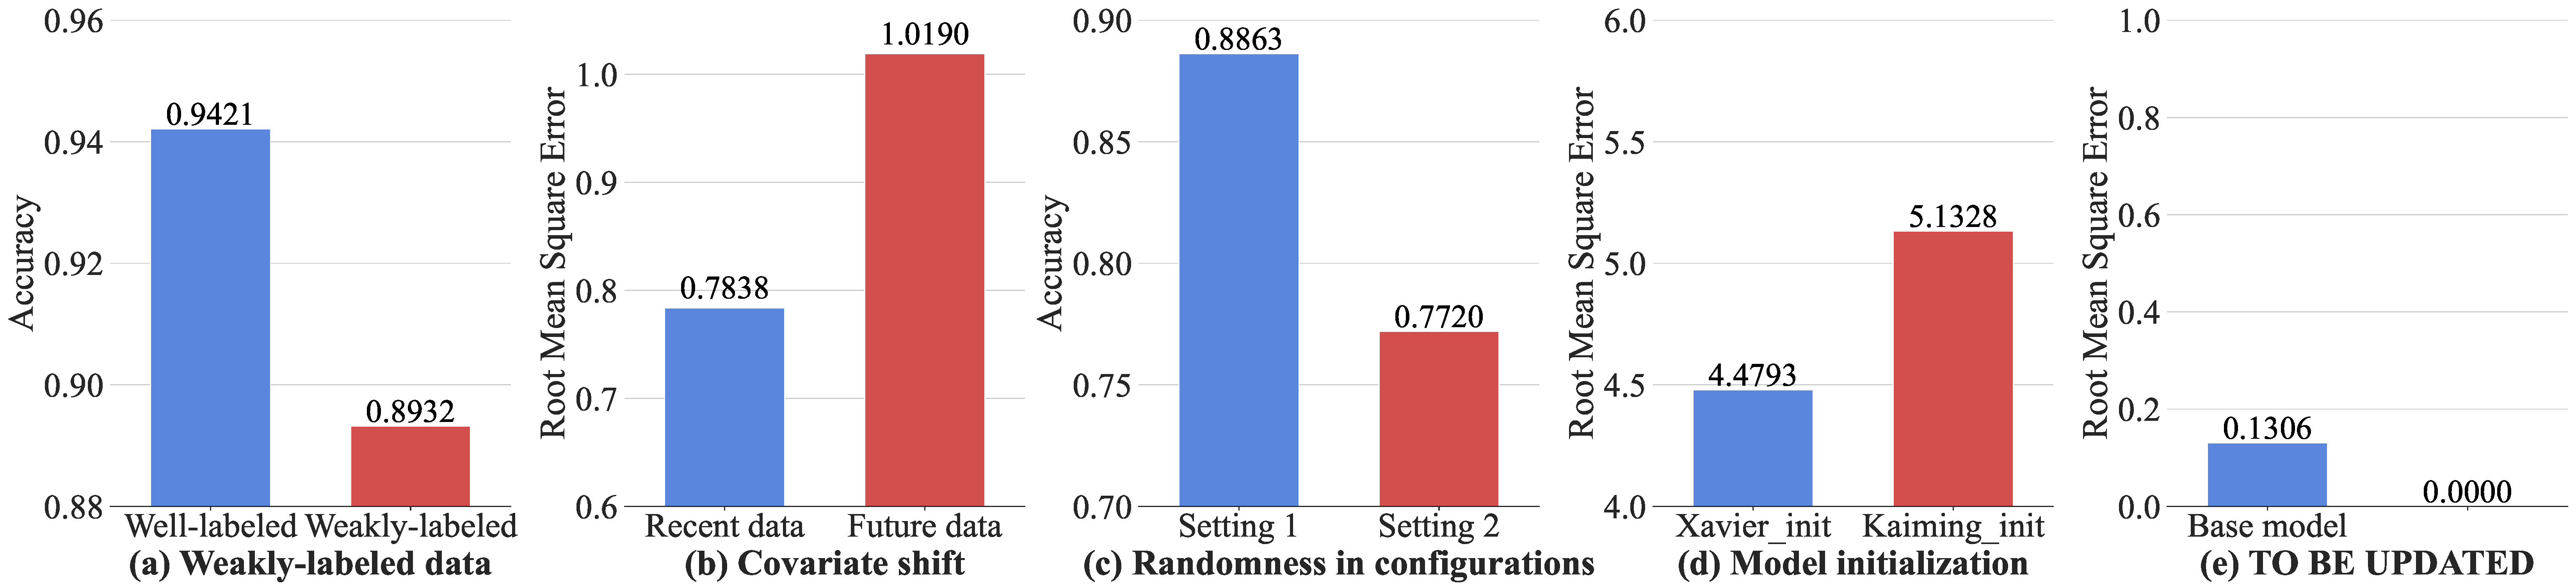
\includegraphics[width=\linewidth]{fig/factors.pdf}
    \caption{Various factors affecting the robustness of deep learning impacting on many of the CSIRO's missions  }
    \label{fig:motivation}
\end{figure}

\noindent
\begin{formal}
{\bf Goal 3:} Model reduction and optimization to  improve training efficiency.
\end{formal}
\noindent
Deep learning models often suffer from redundancy in their network structure, which affects their training efficiency. For example, the over-fitting issue in DNNs~\cite{denil2013predicting} has shown that a large proportion of the configuration parameters are not contributed to the model robustness. 
In this goal, we aim to perform model reduction and optimization to improve training efficiency. Specifically, our novelty lies in robustness-preserved structure transformation to perform network pruning~\cite{han2015learning,luo2017thinet} and  quantize~\cite{ullrich2017soft} through hyperparameter tuning, quantization, parallelism.
The model is reduced and optimized where necessary but preserving the same robustness to boost the adversarial training in \textbf{Goal 2}. Though model reduction (\textbf{Goal 3}) and robustness repair (\textbf{Goal 2}) complement each other, they can be conducted iteratively with one's output as the other's input to continuously improve the overall robustness.
With all that done, we will conduct the final verification to qualitatively certify the underlying DNN model: 
  \noindent
\begin{formal}
{\bf Goal 4:} Quantitative robustness certification of DNN models. 
\end{formal}
\noindent  
Given a repaired and reduced DNN model from \textbf{Goal 2} and \textbf{Goal 3}, our final aim is to conduct precise verification of DNNs using symbolic quantitative certification for the robustness property of the model. 
In the verification of neural networks, a simple yes/no to a verification result about the robustness cannot demonstrate the confidence of the model (e.g., how many perturbed inputs change the model and how much of the deviation of the model has changed). To quantitatively measure and compare the performances of the models by giving in numerous domains would extend the measurement, compared with a threshold deemed with a certain region in a confidence interval. 

